% @Author: AnthonyKenny98
% @Date:   2020-03-19 12:56:13
% @Last Modified by:   AnthonyKenny98
% @Last Modified time: 2020-04-05 13:36:59

\section{Justification of Modelling UAV as Prism}
\label{section:rrt_appendix_modelling}
    While it is possible for a \gls{UAV} to be modelled in precise detail, taking into account its exact shape, more often \glspl{UAV} are modelled as a 3D prism in motion planning problems, for the following reasons:
    \begin{itemize}
    \item It is a rare case that the negative space gained by modelling in such detail is utilised
    \item Representation of drone's configuration is much more complex.
    \item Computing edge collisions is much more computationally intensive.
    \end{itemize}

    % @Author: AnthonyKenny98
% @Date:   2020-04-05 12:55:29
% @Last Modified by:   AnthonyKenny98
% @Last Modified time: 2020-04-05 15:43:13

\begin{figure}[H]
\begin{centering}

\begin{tabular}{cc}
\begin{subfigure}{0.45\linewidth}
    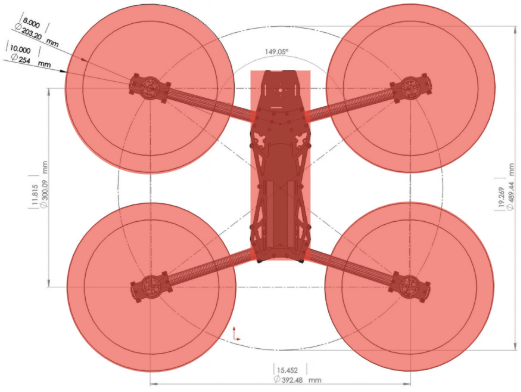
\includegraphics[width=\linewidth]{appendices/rrt/img/DroneNegSpace.png}
    \caption{}
    \label{subfig:dronenegspace}
\end{subfigure}
\begin{subfigure}{0.45\linewidth}
    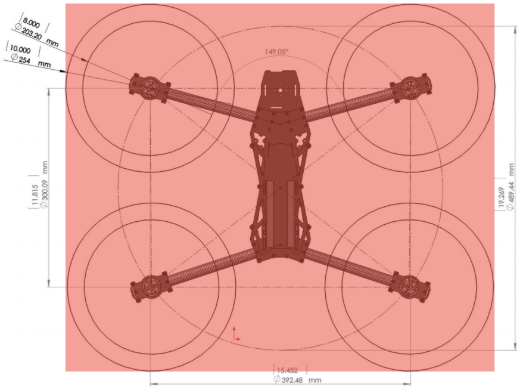
\includegraphics[width=\linewidth]{appendices/rrt/img/DroneRecPrism.png}
    \caption{}
    \label{subfig:dronerecprism}
\end{subfigure}
\end{tabular}
\caption[Modelling a UAV as a Rectangular Prism]{Modelling a \gls{UAV} as a Rectangular Prism. Red highlight demonstrates the model, overlayed over the exact schematic. Figure \ref{subfig:dronenegspace} shows how a drone can be modelled in high detail, but gains little useful free space when compared with Figure \ref{subfig:dronerecprism}, which models a drone as a rectangular prism.\cite{Thingbits}}
\label{fig:dronemodelling}
\end{centering}
\end{figure}

\section{Assessment of Existing RRT Implementations}
\label{section:rrt_appendix_existing_implementations}
    % @Author: AnthonyKenny98
% @Date:   2020-04-05 13:32:41
% @Last Modified by:   AnthonyKenny98
% @Last Modified time: 2020-04-05 13:46:28

\begin{table}[H]
\begin{centering}
\begin{tabular}{|p{0.2\linewidth}|p{0.15\linewidth}|p{0.15\linewidth}|p{0.15\linewidth}|p{0.15\linewidth}|}
\hline
Repository  & Language  &  Workspace Dimension  & Object Model & Algorithmic Correctness \\
\hline
RoboJackets\cite{RoboJackets2019}   & \textcolor{mygreen}{C++}    &       &       & \\
\hline
\end{tabular}
\caption[Evaluation of Existing Open-Source Implementations of RRT]{Evaluation of Existing Open-Source Implementations of RRT. Links to Github repositories can be found in the Bibliography.}
\end{centering}
\end{table}

\section{Justification of K:DIM Ratio}